\documentclass[a4paper,12pt]{article} % тип документа

% Поля страниц
\usepackage[left=2.5cm,right=2.5cm,
    top=2cm,bottom=2cm,bindingoffset=0cm]{geometry}
    
%Пакет дял таблиц   
\usepackage{multirow} 
    
%Отступ после заголовка    
\usepackage{indentfirst}


% Рисунки
\usepackage{floatrow,graphicx,calc}
\usepackage{wrapfig}

%%% Работа с картинками
\usepackage{graphicx}  % Для вставки рисунков
\graphicspath{{images/}{images2/}}  % папки с картинками
\setlength\fboxsep{3pt} % Отступ рамки \fbox{} от рисунка
\setlength\fboxrule{1pt} % Толщина линий рамки \fbox{}
\usepackage{wrapfig} % Обтекание рисунков и таблиц текстом

% Создаёем новый разделитель
\DeclareFloatSeparators{mysep}{\hspace{1cm}}

% Ссылки?
\usepackage{hyperref}
\usepackage[rgb]{xcolor}
\hypersetup{				% Гиперссылки
    colorlinks=true,       	% false: ссылки в рамках
	urlcolor=blue          % на URL
}


%  Русский язык
\usepackage[T2A]{fontenc}			% кодировка
\usepackage[utf8]{inputenc}			% кодировка исходного текста
\usepackage[english,russian]{babel}	% локализация и переносы




% Математика
\usepackage{amsmath,amsfonts,amssymb,amsthm,mathtools}

%%% Дополнительная работа с математикой
\usepackage{amsmath,amsfonts,amssymb,amsthm,mathtools} % AMS
\usepackage{icomma} % "Умная" запятая: $0,2$ --- число, $0, 2$ --- перечисление


% Что-то 
\usepackage{wasysym}


\begin{document}
\begin{center}   
    \hfill \break
	\hfill \break
	\hfill \break
	\large{Лабораторная работа № 4.4.1\\ \hfill \break\Large{Амплитудная диффракционная решетка (гониометр)}}\\\hfill \break\Large{Прамский Илья Б01-203}
\end{center}

\thispagestyle{empty}

\newpage

\textbf{Цель работы:} Знакомство с работой и настройкой гониометра Г5, определение спектральных характеристик амплитудной решётки.

\textbf{В работе используются:} гониометр, дифракционная решётка, ртутная лампа.

\floatsetup[table]{capposition=top}

\section{Теоретическая справка}

Основное соотношение приближенной теории дифракционной решётки:

	\begin{equation}
	d\sin \varphi_m = m\lambda.
 \label{main}
	\end{equation}
 
Угловая дисперсия $D$ характеризует угловое расстояние между близкими спектральными линиями:
	\begin{equation}
	D = \frac{d\varphi}{d\lambda} = \frac{m}{d \cos \varphi}=\frac{m}{\sqrt{d^{2}-m^{2} \lambda^{2}}}.
	\label{Dispersion}
	\end{equation}

Рассмотрим изображения спектра для двух узких спектральных линий с длинами волн $\lambda$ и $\lambda+\delta\lambda$. Для минимального значения $\lambda+\delta\lambda$, которое может быть определено по результатам измерений, вводят важнейшую характеристику спектрального прибора — разрешающую способность:

\begin{equation}
    R=\frac{\lambda}{\delta\lambda} = \frac{\varphi}{\delta \varphi}.
\end{equation}


\section{Экспериментальная установка}

\subsection{Устройство гониометра}

Гониометр служит для точного измерения углов и находит широкое применение в оптических лабораториях. С помощью гониометра можно определять показатели преломления и преломляющие углы призм и кристаллов, исследовать параметры дифракционных решёток, измерять длины волн спектральных линий и т. Д.

Оптическая схема гониометра представлена на рис. 1а. Свет от источника $S$ проходит через коллиматор (устройство, дающее параллельный пучок, состоящее из щели 1 и объектива 5 ) и преобразуется призмой или решёткой в набор параллельных пучков, каждый из которых соответствует определённой длине волны.

\begin{figure}[H]
    \centering
    \includegraphics[scale=0.4]{2023_04_02_a48ae02e429ba186bcd7g-1(1)}

    \includegraphics[scale=0.4]{2023_04_02_a48ae02e429ba186bcd7g-1}\\
    {Рис. 2: Автоколлимационное устройство}
    \label{fig:my_label}
\end{figure}

Параллельные пучки собираются в фокальной плоскости объектива 9 зрительной трубы и рассматриваются глазом через окуляр 14. При освещении щели ртутной лампой, дающей дискретный спектр, в фокальной плоскости видны отдельные линии - цветные изображения входной щели (см. рис. 4 и таблицу 1).

Внешний вид гониометра представлен на рис. 16 и 1в. Коллиматор 3, столик 7 и алидада 17 со зрительной трубой 12 крепятся на массивном основании 23. На столике 7 размещаются исследуемые объекты. Коллиматор закреплён неподвижно, а столик и алидада с трубой могут вращаться вокруг вертикальной оси.

Ширину коллиматорной щели можно менять от 0 до 2-х мм при помощи микрометрического винта 2 , высоту - от 0 до 2-х см - при помощи диафрагмы с треугольным вырезом («ласточкин хвост»), надетой на щель. Винт 4 служит для перемещения объектива 5 - настройки коллиматора на параллельный пучок.

Зрительная труба 12 состоит из объектива 9 и окуляра 14 с автоколлимационным устройством 13. Объективы коллиматора и зрительной трубы одинаковы. Фокусировка трубы производится винтом 11. Наклон коллиматора и зрительной трубы к горизонтальной оси изменяется винтами 6 и 10 соответственно.

Схема окуляра О зрительной трубы с автоколлимационным устройством приведена на рис. 2а. Свет от лампы Л проходит через защитную стеклянную пластинку П и попадает на автоколлимационную сетку А, содержащую две взаимно перпендикулярные щели. Свет, прошедший через сетку А (светящийся крест - рис. 2б), попадает на две прямоугольные призмы $P$ и отражается от гипотенузной грани, на которую нанесён полупрозрачный слой с коэффициентом отражения $50 \%$.

Для юстировки гониометра на столик ставится предмет с плоской отражающей поверхностью. После отражения от неё 

A)
\begin{center}
    \includegraphics[scale=0.2]{2023_04_02_a48ae02e429ba186bcd7g-2}
\end{center}


Б)

\begin{center}
\includegraphics[scale=0.2]{2023_04_02_a48ae02e429ba186bcd7g-2(2)}
\end{center}

B)

\begin{center}
\includegraphics[scale=0.2]{2023_04_02_a48ae02e429ba186bcd7g-2(1)}

Рис. 1. Оптическая схема и внешний вид гониометра

\end{center}

 параллельный пучок лучей возвращается назад в зрительную трубу и собирается в фокальной плоскости объектива. В этом случае светящийся автоколлимационный крест можно увидеть через окуляр зрительной трубы. Кроме того, в окуляре имеется ещё одна сетка C, на которой изображён чёрный отсчётный крест (рис. 2в). Совмещённые изображения обоих крестов рассматриваются через окулярные линзы О. Резкость видимого изображения отсчётного креста регулируется вращением оправы окуляра трубы.

Обе сетки окуляра, А и C (рис. 2а), расположены на строго одинаковых расстояниях от гипотенузных граней призмы $P$, поэтому их одновременное наблюдение в окуляре возможно только при совпадении фокальных плоскостей объектива и окуляра (труба настроена на бесконечность).

Важнейшим узлом гониометра является устройство, служащее для отсчёта угла поворота зрительной трубы вокруг вертикальной оси, проходящей через центр столика. На этой оси крепится прозрачное кольцо (лимб), расположенное в корпусе прибора. На поверхности лимба нанесена шкала с делениями. Лимб разделён на $3 \times 360=1080$ делений. Цена деления $20^{\prime}$, оцифровка делений произведена через $1^{\circ}$. Шкалу лимба можно наблюдать через окуляр отсчётного устройства 16 при включённой подсветке (тумблер 22). Резкость изображения шкалы регулируется вращением оправы окуляра 15.

Оптическая система отсчётного устройства собрана так, что через окуляр можно наблюдать изображения штрихов двух диаметрально противоположных участков лимба, причём одно изображение прямое, а другое обратное (рис. 3). Кроме того, оптическая система позволяет перемещать эти изображения друг относительно друга, оставляя в покое как лимб, так и алидаду со зрительной трубой. Это перемещение штрихов измеряется при помощи оптического микрометра. Шкала микрометра рассчитана таким образом, что при перемещении её на 600 делений верхнее изображение штрихов лимба смещается относительно нижнего на 10'. Следовательно, цена деления шкалы микрометра $1^{\prime \prime}$.

Поле зрения отсчётного микроскопа приведено на рис. 3. В левом окне наблюдаются изображения диаметрально противоположных участков лимба и вертикальный штрих для отсчёта градусов, в правом - деления шкалы оптического микрометра и горизонтальная риска $R$ для отсчёта минут и секунд.

Для удобства экспериментатора в гониометре предусмотрено несколько вариантов относительного вращения столика, алидады со зрительной трубой и лимба.
Отсчётное устройство гониометра обеспечивает точность измерения угла не хуже $5^{\prime \prime}$.

\section{Ход работы}
В работе используется дифракционная решётка с периодом $d = 2$ мкм(500 штрихов на миллиметр). Значения длин волн будем брать из таблицы характеристик спектра ртутной лампы ДРШ(из методический материалов к лабораторной работе)

Для начала опишем измерения, проведённые во время эксперимента для оценки  соблюдения всех правил его выполнения, а затем перейдём к исследованиям зависимостей и тому подобному(обработке результатов).
После настройки гониометра и установки ртутной лампы, проверим, что эксперимент проводится правильно. Убедимся в этом при помощи формулы (1) для одного из цветов. Так, для зелёного получилось $\alpha = 16^\circ 4' 5''$. Тогда получается $d \cdot \sin \alpha \simeq 550$ нм(заметим, что у зелёного света $\lambda = 495-570$ нм).

Теперь перейдём к обработке результатов эксперимента.

Рассчитав углы дифракции для $\pm 1$ порядка, исследуем зависимость $\sin \varphi_m = f(\lambda)$. Данные занесём в таблицу и построим график зависимости. 

\begin{table}[H]
	\centering
	\begin{tabular}{c|c|c|c}
	$\varphi_1$ & $\varphi_{-1}$ & $\sigma_\varphi$ & $\lambda$, нм 	\\
	$13^\circ 27' 50''$ & $-12^\circ 35' 50''$ & $30''$ & 404,7 \\
	$15^\circ 16' 30''$ & $-14^\circ 11' 40''$ & $30''$ & 491,6 \\
	$16^\circ 4'  30''$ & $-15^\circ 45' 50''$ & $30''$ & 546,1 \\
	$17^\circ 5'  10''$ & $-16^\circ 37' 10''$ & $30''$ & 577,0 \\
	$17^\circ 9'  10''$ & $-17^\circ 0'  0''$  & $30''$ & 579,1 \\
	\end{tabular}
\end{table}

\begin{figure}[H]
    \centering
    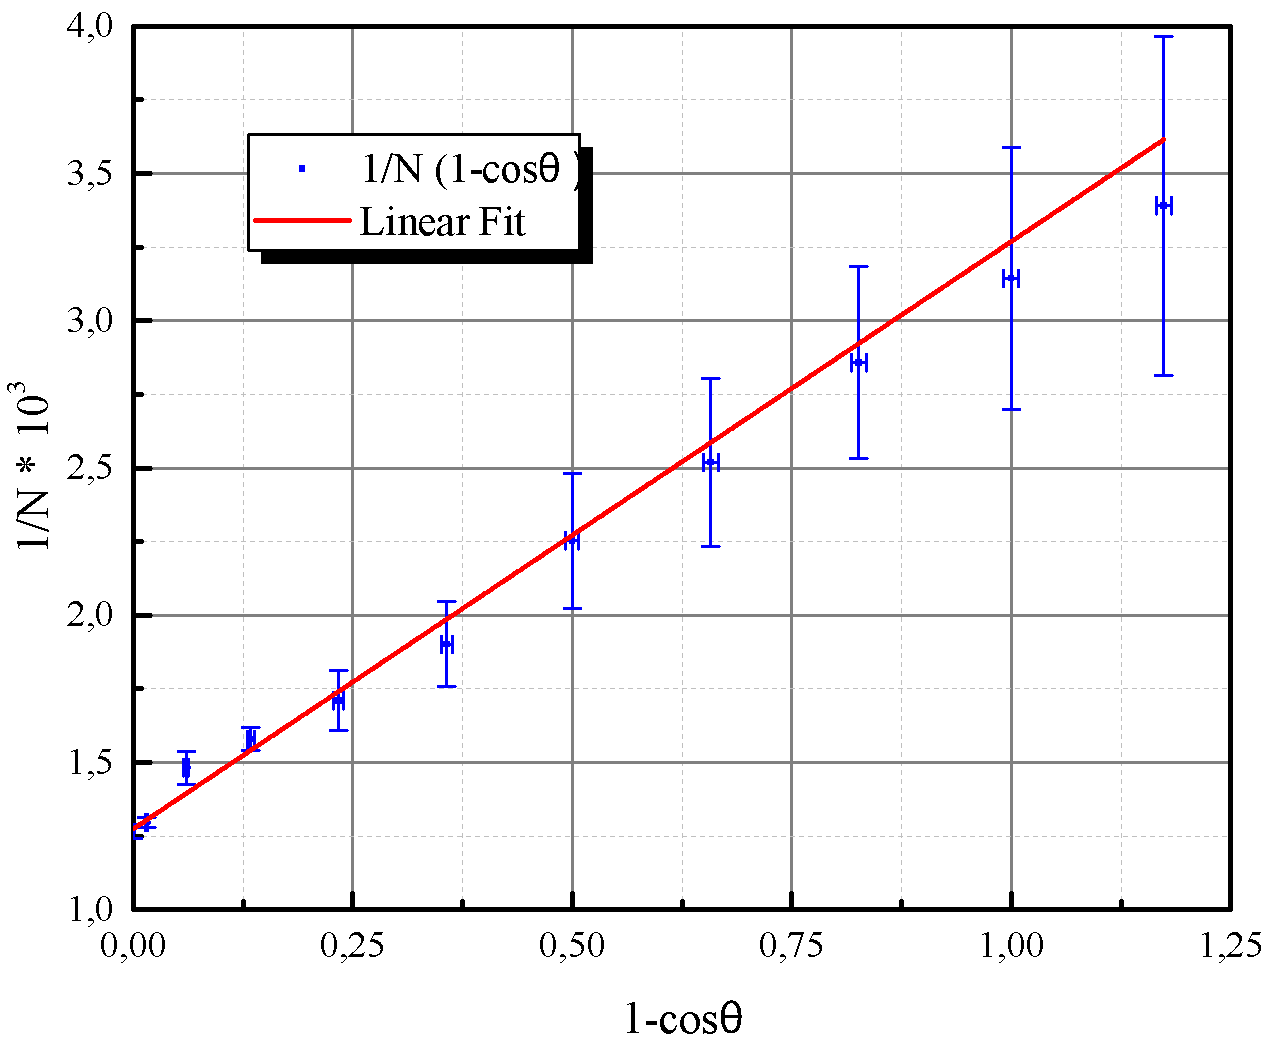
\includegraphics[scale=0.8]{graph1}
\end{figure}

По углу наклона оценим значение d. $k = 0,0004 \pm 0,00003$ $\text{нм}^{-1}$.

$d = \frac{1}{k} = 2,50 \pm 0,18$ мкм.

Теперь измерим угловые координаты желтых пар на тех порядках, которые будут видны на гониометре, а также вычислим для каждой угловую дисперсию. Полученные данные занесём в таблицу и по ним сравним зависимость $D = f(m)$ с теоретической (2). $\Delta \lambda = 2,1$ нм = 21 \r{A}.

\begin{table}[H]
	\centering
	\begin{tabular}{c|c|c|c|c|c}
	 m & $\varphi_1$ & $\varphi_2$ & $\Delta \varphi$ & D, $10^{-5}$ $\text{\r{A}}^{-1}$ & $\sigma_D$ \\
	 1 & $17^\circ 5' 6''$     & $17^\circ 9' 11''$   & $245''$  &  5,7 & 0,3 \\
 	-1 & $-16^\circ 37' 12''$  & $-16^\circ 42' 8''$  & $-296''$ & -6,8 & 0,3 \\
 	 2 & $40^\circ 59' 59''$   & $41^\circ 9' 12'' $  & $553''$  &  12,8 & 0,6\\
 	-2 & $-33^\circ 26' 47''$  & $-33^\circ 39' 1''$  & $-734''$ & -16,9 & 0,8\\
 	-3 & $-52^\circ 30' 51''$  & $-52^\circ 40' 24''$ & $-573''$ & -13,2 & 0,7\\
	
	\end{tabular}
\end{table}

\begin{figure}[H]
	\centering
	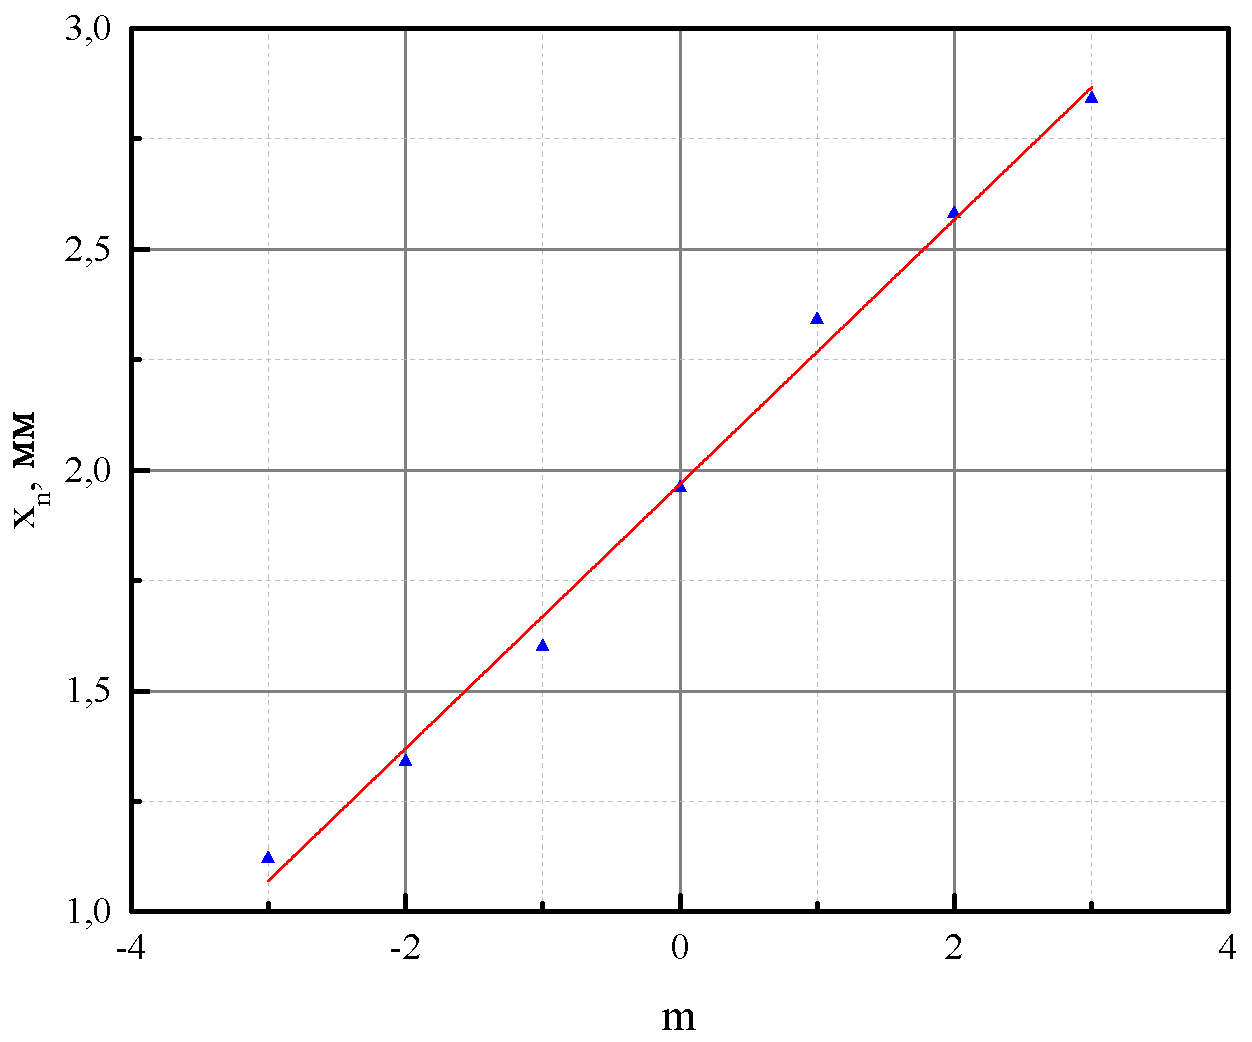
\includegraphics[scale=0.8]{graph2}
\end{figure}

Как видно из графика, большая часть точек находится вблизи значений, полученных теоретически(помимо точки порядка -3, что можно сослать на плохую видимость полос на этом порядке).

Теперь по угловой ширине одной из полос определим разрещающую способность, а затем с её помощью оценим число рабочих штрихов, а также размер освещённой части решётки. Так, измеренная угловая ширина одной из жёлтых полос первого порядка($\varphi = 17^\circ 5' 10'')$ составила $\delta \varphi = 2' 5'' = 125''$. Тогда получается $R \simeq 492$, а количество рабочих штрихов $N = R\cdot m = 492$, размер освещённой части $l = N \cdot \simeq 984$ мкм.


$m_\text{ж} \lambda_\text{ж} = m_\text{ф} \lambda_\text{ф}$ при слиянии. Тогда получается $m_\text{ж} = 7, m_\text{ф} = 10$.

\section{Вывод}
В ходе работы был изучен способ работы и настройки гониометра. Также с его помощью была проверена справедливость формулы (1), затем было получено значение периода дифракционной решётки($d = 2,50 \pm 0,18$ мкм), которое находится достаточно близко к истинному значению($d = 2$ мкм). Помимо этого, была также получена зависимость угловой дисперсии от порядка дифракции, которая затем, при сравнении с теоретической зависимостью, в некоторых точках даже совпала с ней(при этом в одной точке($m=-3$) у нас явная ошибка, связанная с тем, что на данном порядке жёлтая полоса уже практически вышла за пределы поля зрения). В конце концов, было получено значение разрешающей способности и при помощи неё затем оценены количество рабочих штрихов(492) и размер освещённой части(984 мкм).

\end{document}
